\documentclass[10pt]{article}
\usepackage[polish]{babel}
\usepackage[utf8]{inputenc}
\usepackage[T1]{fontenc}
\usepackage{amsmath}
\usepackage{amsfonts}
\usepackage{amssymb}
\usepackage[version=4]{mhchem}
\usepackage{stmaryrd}
\usepackage{graphicx}
\usepackage[export]{adjustbox}
\graphicspath{ {./images/} }

\title{OD SZKOLNIAKA DO ŻAKA }

\author{}
\date{}


\begin{document}
\maketitle
\section*{klasy 7 i 8 szkoły podstawowej}
rok szkolny 2022/2023\\
Zadania - etap II

Zadanie 1. Wykaż, że liczba 8-cyfrowa postaci \(A B A B A B A B\) jest podzielna przez 101.

Zadanie 2. Suma cyfr liczby 3-cyfrowej podzielnej przez 5 jest równa 17. Jeżeli zapiszemy cyfry tej liczby w przeciwnej kolejności to otrzymamy liczbę o 99 większą od początkowej. Wyznacz te liczby.

Zadanie 3. Ile jest liczb naturalnych większych od 200 i nie większych od 400, które są:\\
a). podzielne przez 3 i 5 .\\
b). podzielne przez 3 lub podzielne przez 5.

Zadanie 4. Na rysunku przedstawiono trapez \(A B C D\) oraz trójkąt \(A F D\). Punkt \(E\) leży w połowie odcinka \(B C\). Uzasadnij, że pole trapezu \(A B C D\) i pole trójkąta \(A F D\) są równe.\\
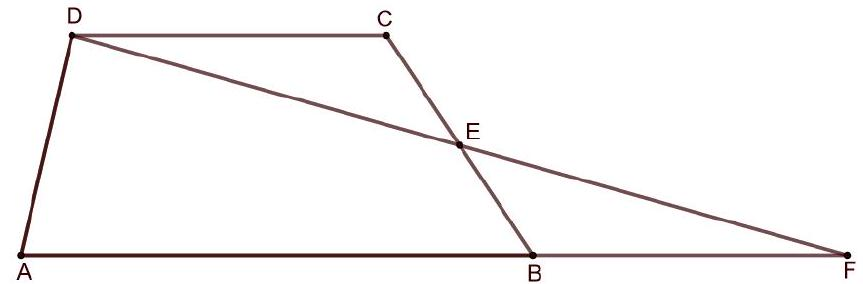
\includegraphics[max width=\textwidth, center]{2024_11_21_7fff4e7075cc1bd990c9g-1}

Zadanie 5. Na rysunku przedstawiono dwa równoległoboki \(A B C D\) i \(A B E F\). Uzasadnij, że czworokąty CDAG oraz EFGB mają równe pola.\\
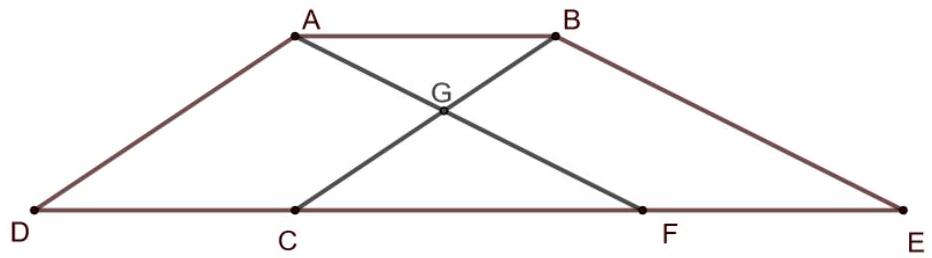
\includegraphics[max width=\textwidth, center]{2024_11_21_7fff4e7075cc1bd990c9g-1(1)}


\end{document}